% Options for packages loaded elsewhere
% Options for packages loaded elsewhere
\PassOptionsToPackage{unicode}{hyperref}
\PassOptionsToPackage{hyphens}{url}
\PassOptionsToPackage{dvipsnames,svgnames,x11names}{xcolor}
%
\documentclass[
  letterpaper,
  DIV=11,
  numbers=noendperiod]{scrreprt}
\usepackage{xcolor}
\usepackage{amsmath,amssymb}
\setcounter{secnumdepth}{5}
\usepackage{iftex}
\ifPDFTeX
  \usepackage[T1]{fontenc}
  \usepackage[utf8]{inputenc}
  \usepackage{textcomp} % provide euro and other symbols
\else % if luatex or xetex
  \usepackage{unicode-math} % this also loads fontspec
  \defaultfontfeatures{Scale=MatchLowercase}
  \defaultfontfeatures[\rmfamily]{Ligatures=TeX,Scale=1}
\fi
\usepackage{lmodern}
\ifPDFTeX\else
  % xetex/luatex font selection
\fi
% Use upquote if available, for straight quotes in verbatim environments
\IfFileExists{upquote.sty}{\usepackage{upquote}}{}
\IfFileExists{microtype.sty}{% use microtype if available
  \usepackage[]{microtype}
  \UseMicrotypeSet[protrusion]{basicmath} % disable protrusion for tt fonts
}{}
\makeatletter
\@ifundefined{KOMAClassName}{% if non-KOMA class
  \IfFileExists{parskip.sty}{%
    \usepackage{parskip}
  }{% else
    \setlength{\parindent}{0pt}
    \setlength{\parskip}{6pt plus 2pt minus 1pt}}
}{% if KOMA class
  \KOMAoptions{parskip=half}}
\makeatother
% Make \paragraph and \subparagraph free-standing
\makeatletter
\ifx\paragraph\undefined\else
  \let\oldparagraph\paragraph
  \renewcommand{\paragraph}{
    \@ifstar
      \xxxParagraphStar
      \xxxParagraphNoStar
  }
  \newcommand{\xxxParagraphStar}[1]{\oldparagraph*{#1}\mbox{}}
  \newcommand{\xxxParagraphNoStar}[1]{\oldparagraph{#1}\mbox{}}
\fi
\ifx\subparagraph\undefined\else
  \let\oldsubparagraph\subparagraph
  \renewcommand{\subparagraph}{
    \@ifstar
      \xxxSubParagraphStar
      \xxxSubParagraphNoStar
  }
  \newcommand{\xxxSubParagraphStar}[1]{\oldsubparagraph*{#1}\mbox{}}
  \newcommand{\xxxSubParagraphNoStar}[1]{\oldsubparagraph{#1}\mbox{}}
\fi
\makeatother


\usepackage{longtable,booktabs,array}
\usepackage{calc} % for calculating minipage widths
% Correct order of tables after \paragraph or \subparagraph
\usepackage{etoolbox}
\makeatletter
\patchcmd\longtable{\par}{\if@noskipsec\mbox{}\fi\par}{}{}
\makeatother
% Allow footnotes in longtable head/foot
\IfFileExists{footnotehyper.sty}{\usepackage{footnotehyper}}{\usepackage{footnote}}
\makesavenoteenv{longtable}
\usepackage{graphicx}
\makeatletter
\newsavebox\pandoc@box
\newcommand*\pandocbounded[1]{% scales image to fit in text height/width
  \sbox\pandoc@box{#1}%
  \Gscale@div\@tempa{\textheight}{\dimexpr\ht\pandoc@box+\dp\pandoc@box\relax}%
  \Gscale@div\@tempb{\linewidth}{\wd\pandoc@box}%
  \ifdim\@tempb\p@<\@tempa\p@\let\@tempa\@tempb\fi% select the smaller of both
  \ifdim\@tempa\p@<\p@\scalebox{\@tempa}{\usebox\pandoc@box}%
  \else\usebox{\pandoc@box}%
  \fi%
}
% Set default figure placement to htbp
\def\fps@figure{htbp}
\makeatother





\setlength{\emergencystretch}{3em} % prevent overfull lines

\providecommand{\tightlist}{%
  \setlength{\itemsep}{0pt}\setlength{\parskip}{0pt}}



 


\KOMAoption{captions}{tableheading}
\makeatletter
\@ifpackageloaded{bookmark}{}{\usepackage{bookmark}}
\makeatother
\makeatletter
\@ifpackageloaded{caption}{}{\usepackage{caption}}
\AtBeginDocument{%
\ifdefined\contentsname
  \renewcommand*\contentsname{Table of contents}
\else
  \newcommand\contentsname{Table of contents}
\fi
\ifdefined\listfigurename
  \renewcommand*\listfigurename{List of Figures}
\else
  \newcommand\listfigurename{List of Figures}
\fi
\ifdefined\listtablename
  \renewcommand*\listtablename{List of Tables}
\else
  \newcommand\listtablename{List of Tables}
\fi
\ifdefined\figurename
  \renewcommand*\figurename{Figure}
\else
  \newcommand\figurename{Figure}
\fi
\ifdefined\tablename
  \renewcommand*\tablename{Table}
\else
  \newcommand\tablename{Table}
\fi
}
\@ifpackageloaded{float}{}{\usepackage{float}}
\floatstyle{ruled}
\@ifundefined{c@chapter}{\newfloat{codelisting}{h}{lop}}{\newfloat{codelisting}{h}{lop}[chapter]}
\floatname{codelisting}{Listing}
\newcommand*\listoflistings{\listof{codelisting}{List of Listings}}
\makeatother
\makeatletter
\makeatother
\makeatletter
\@ifpackageloaded{caption}{}{\usepackage{caption}}
\@ifpackageloaded{subcaption}{}{\usepackage{subcaption}}
\makeatother
\usepackage{bookmark}
\IfFileExists{xurl.sty}{\usepackage{xurl}}{} % add URL line breaks if available
\urlstyle{same}
\hypersetup{
  pdftitle={Nizham Rafa Lazuardi},
  pdfauthor={18224049 Nizham Rafa Lazuardi},
  colorlinks=true,
  linkcolor={blue},
  filecolor={Maroon},
  citecolor={Blue},
  urlcolor={Blue},
  pdfcreator={LaTeX via pandoc}}


\title{Nizham Rafa Lazuardi}
\usepackage{etoolbox}
\makeatletter
\providecommand{\subtitle}[1]{% add subtitle to \maketitle
  \apptocmd{\@title}{\par {\large #1 \par}}{}{}
}
\makeatother
\subtitle{Portfolio Asesmen II-2100 KIPP}
\author{18224049 Nizham Rafa Lazuardi}
\date{2025-09-15}
\begin{document}
\maketitle

\renewcommand*\contentsname{Table of contents}
{
\hypersetup{linkcolor=}
\setcounter{tocdepth}{2}
\tableofcontents
}

\bookmarksetup{startatroot}

\chapter*{Selamat Berjumpa}\label{selamat-berjumpa}
\addcontentsline{toc}{chapter}{Selamat Berjumpa}

\markboth{Selamat Berjumpa}{Selamat Berjumpa}

Saya \textbf{Nizham Rafa Lazuardi}, mahasiswa \textbf{Sekolah Teknik
Elektro dan Informatika ITB}, program \textbf{Sistem dan Teknologi
Informasi}.\\
Saya lahir dan besar di Indonesia, saat ini sedang menapaki perjalanan
sebagai \textbf{game designer dan creative technologist} yang tertarik
pada bagaimana teknologi bisa memunculkan \emph{rasa
manusiawi}---seperti empati, keingintahuan, dan harapan---di dalam
sebuah sistem interaktif.

Saya suka menulis, mendesain, dan merenung.\\
Ketiganya sering bercampur jadi satu: dari jurnal refleksi sederhana,
menjadi ide game kecil, lalu tumbuh jadi sistem yang ingin saya bagi
dengan orang lain.\\
Bagi saya, desain bukan hanya tentang fungsi atau visual, tapi tentang
\textbf{cerita dan makna yang bisa dirasakan pemain}.

Sejak kuliah, saya banyak belajar bahwa kreativitas tidak selalu datang
dari inspirasi besar, tapi dari keberanian mencoba walau gagal.\\
Saya pernah merasa tidak berbakat, bahkan sempat ingin berhenti
berkarya.\\
Namun dari titik itu saya belajar, bahwa setiap langkah kecil tetap
berarti---asal dilakukan dengan jujur dan konsisten.

Karya dan refleksi saya dapat ditemukan di portofolio ini, serta di
halaman-halaman tugas seperti \textbf{``My Song for You''}, \textbf{``My
Stories for You''}, dan \textbf{``My SHAPE''}.\\
Masing-masing menjadi catatan perjalanan saya untuk mengenali diri,
memperbaiki langkah, dan berbagi sesuatu yang bisa menguatkan orang lain
juga.

Oh, dan ya --- saya juga punya kebiasaan aneh: menulis catatan tengah
malam sambil memikirkan ide game yang mungkin tidak akan pernah
selesai.\\
Tapi siapa tahu, suatu hari nanti salah satunya akan hidup dan membuat
seseorang tersenyum.\\
Kalau itu terjadi, mungkin semua rasa gagal itu akhirnya tidak sia-sia.

Terima kasih sudah berkunjung --- semoga halaman ini membawa sedikit
inspirasi, atau sekadar rasa tenang yang meneguhkan.

\begin{quote}
``Kita semua sedang belajar melangkah, satu `better step' pada satu
waktu.''
\end{quote}

\bookmarksetup{startatroot}

\chapter{UTS-1 All About Me}\label{uts-1-all-about-me}

\begin{figure}[H]

{\centering 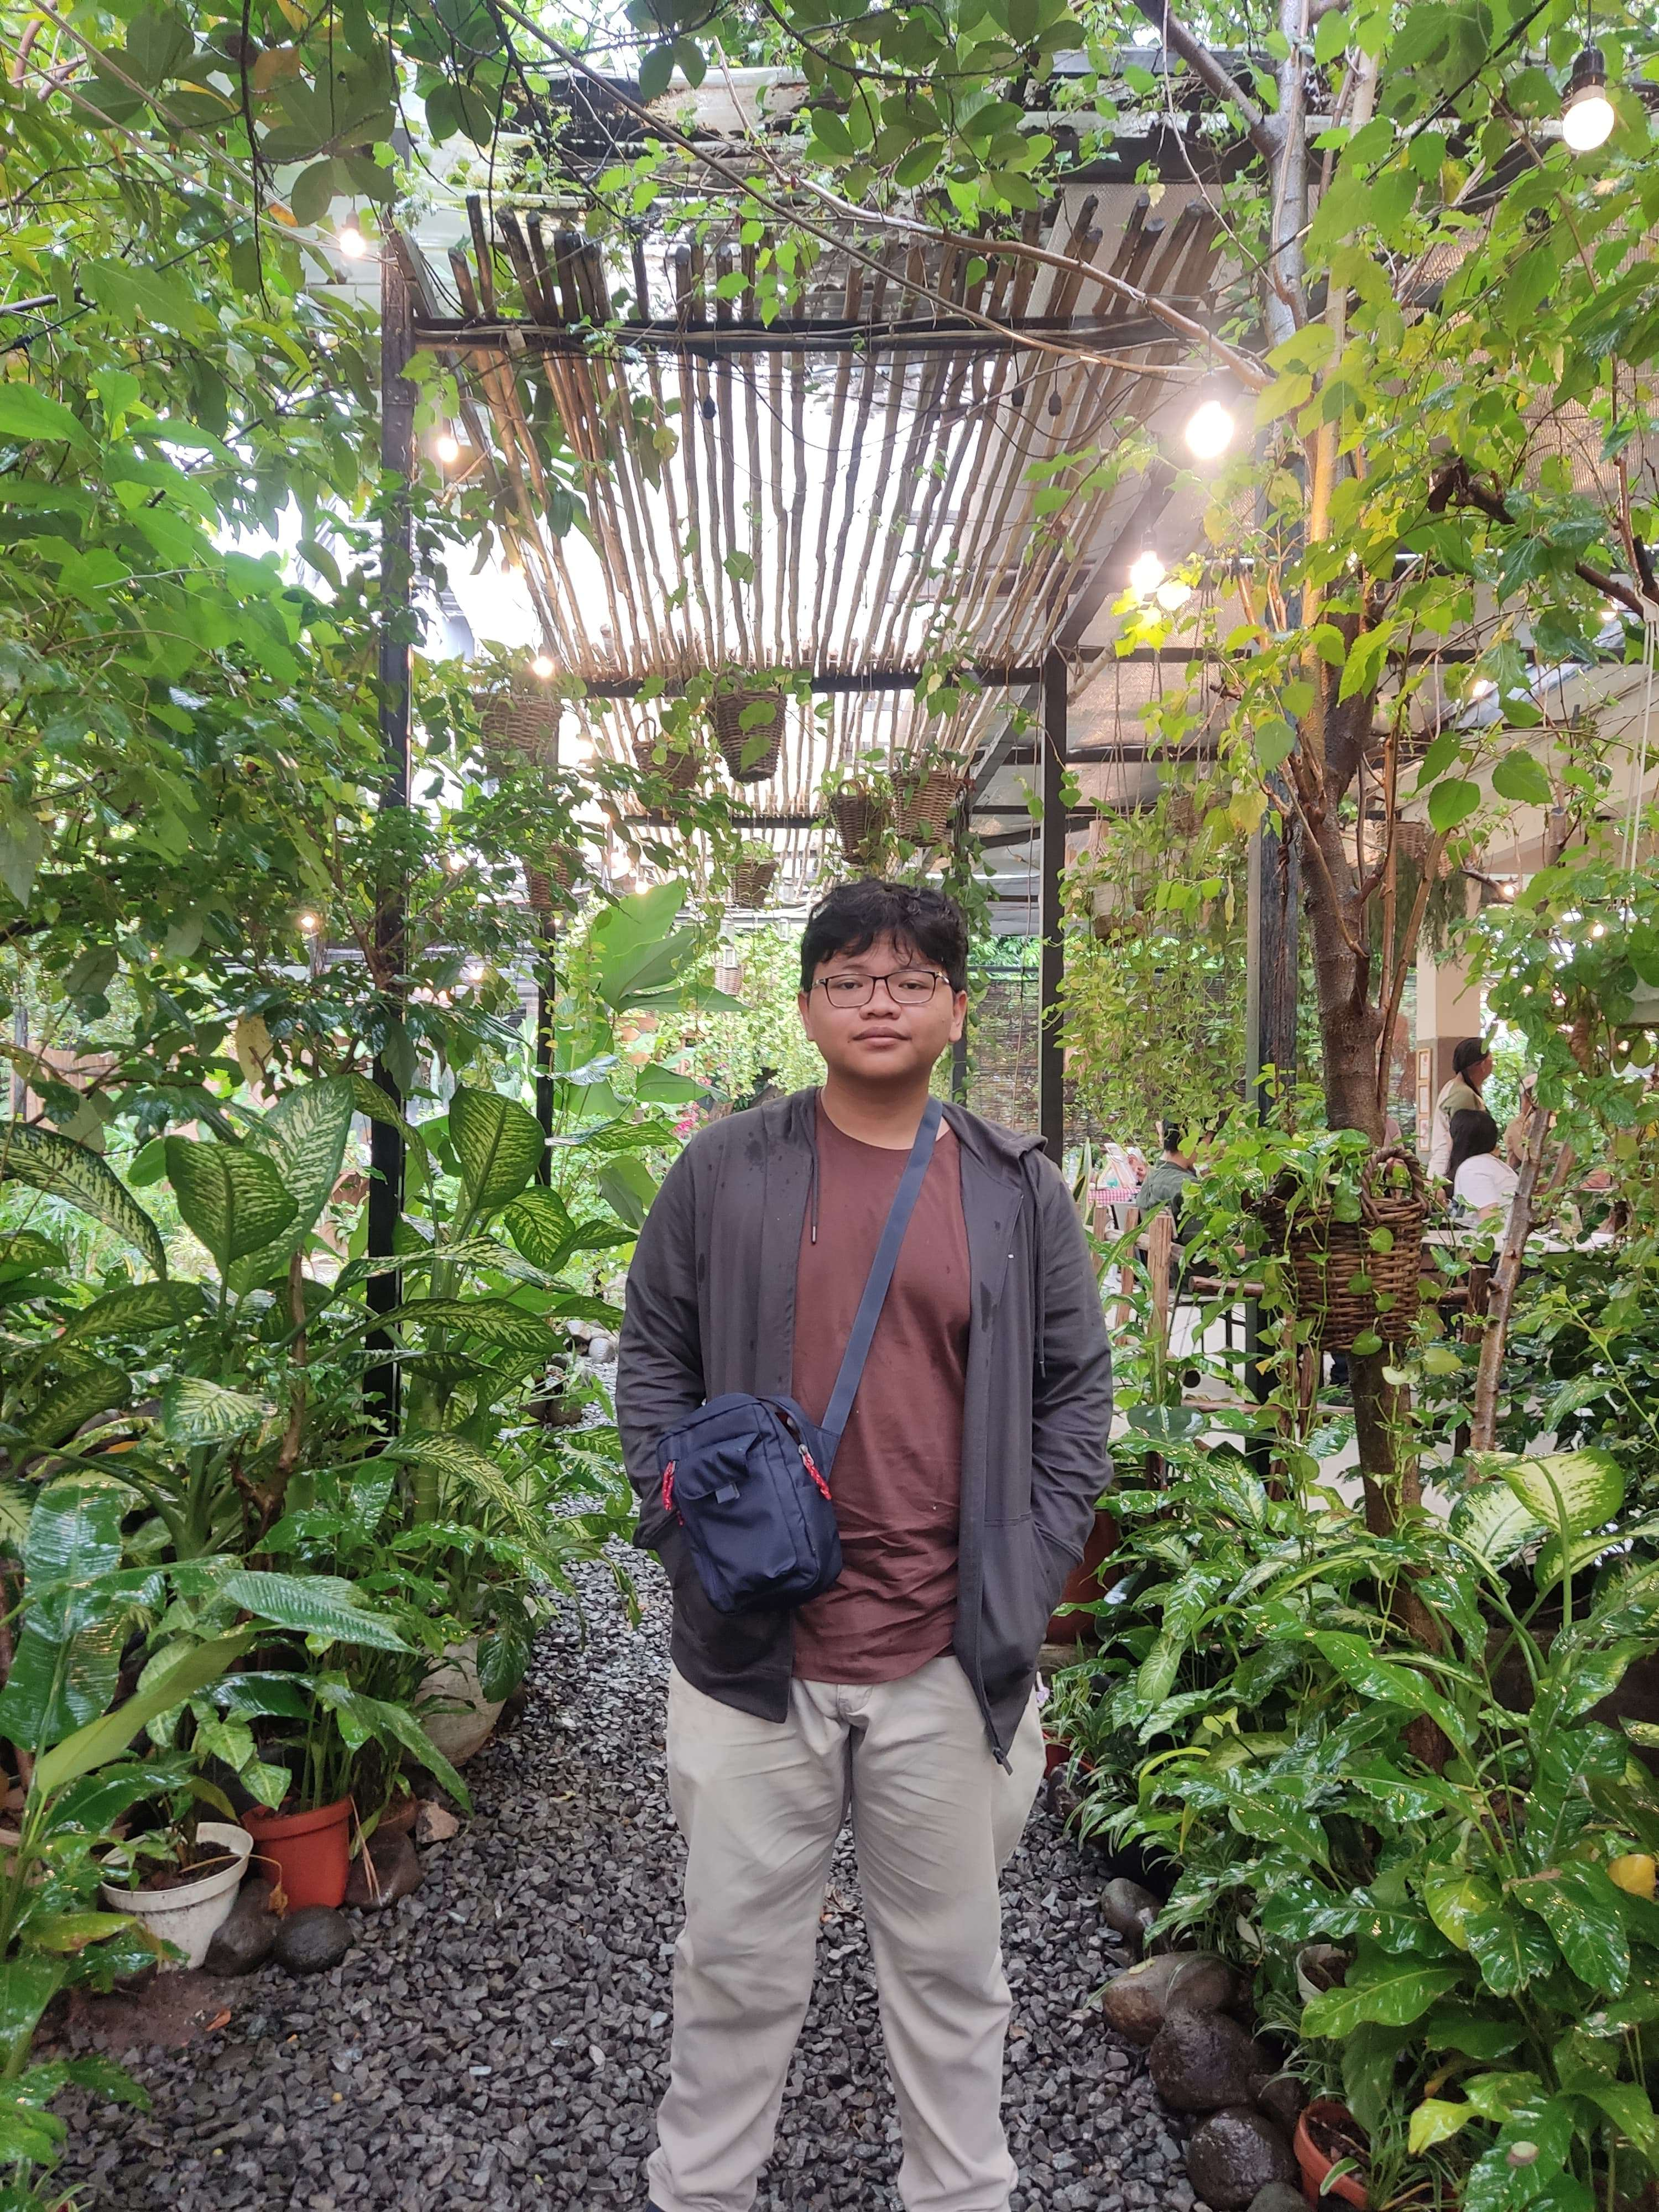
\includegraphics[width=9.5\linewidth,height=\textheight,keepaspectratio]{All_About_me/../images/nizham.jpg}

}

\caption{About Me}

\end{figure}%

\textbf{Nizham Rafa Lazuardi} adalah mahasiswa \textbf{Sistem dan
Teknologi Informasi ITB} yang sedang menapaki dunia yang seimbang antara
logika dan kreativitas. Ia tertarik pada \textbf{game development,
UI/UX, dan artificial intelligence}, tiga bidang yang menurutnya
sama-sama menantang dan menyenangkan karena semua berbicara tentang satu
hal: \textbf{bagaimana manusia berinteraksi dengan sistem yang mereka
ciptakan sendiri.}

Lahir dan besar di Indonesia, Nizham saat ini menempuh semester awal di
STEI-K ITB. Di luar kuliah, ia suka mengulik ide-ide game yang ``nggak
biasa'', misalnya memadukan konsep klasik dengan mekanik baru yang
menuntut pemain berpikir strategis sekaligus reflektif. Ia percaya bahwa
permainan terbaik bukan hanya menghibur, tetapi juga membuat pemain
\emph{merasakan sesuatu tentang dirinya sendiri.}

Di dunia nyata, Nizham dikenal sebagai seseorang yang suka berpikir
dalam, kadang terlalu dalam hingga lupa makan siang. Tapi, bagi dia,
berpikir adalah bentuk hiburan yang tak kalah menarik dari bermain game.

Instagram? Masih kosong. Blog? Sedang dalam tahap ``nanti kalau
sempat.'' Tapi pikirannya selalu aktif di mana pun ia berada.

Apa gagasan yang sedang ia pikirkan?

\begin{center}\rule{0.5\linewidth}{0.5pt}\end{center}

\section{\texorpdfstring{\textbf{Kisah yang Membentuk Diri Saya: Antara
Pixel, Makna, dan
Manusia}}{Kisah yang Membentuk Diri Saya: Antara Pixel, Makna, dan Manusia}}\label{kisah-yang-membentuk-diri-saya-antara-pixel-makna-dan-manusia}

Manusia menciptakan cerita untuk memahami dunia, dan mungkin itu alasan
mengapa saya jatuh cinta pada dunia game. Game adalah bentuk narasi
interaktif: pemain membuat pilihan, menanggung konsekuensi, dan akhirnya
menulis kisahnya sendiri. Di sanalah saya sadar bahwa hidup pun bekerja
dengan cara yang sama.

Bagi saya, belajar komunikasi interpersonal seperti \emph{debugging}
hubungan antar manusia. Kita semua punya ``kode sosial'' yang kompleks,
dan terkadang kesalahan kecil dalam ekspresi bisa membuat seluruh sistem
interaksi ``crash.'' Tapi justru di situ letak seninya: memahami orang
lain bukanlah tentang menjadi sempurna, melainkan tentang \emph{belajar
membaca sinyal-sinyal halus yang sering kita abaikan.}

Saya melihat bahwa keahlian berbicara dan mendengar seimbang seperti
desain UI yang baik: intuitif, responsif, dan punya \emph{feedback loop}
yang jujur. Sebuah percakapan yang sehat, seperti game yang baik,
membuat kita ingin terus bermain, bukan cepat keluar.

\begin{center}\rule{0.5\linewidth}{0.5pt}\end{center}

\subsection{\texorpdfstring{\textbf{1. Diri Saya dan ``Tiga Lapisan
Game''
Kehidupan}}{1. Diri Saya dan ``Tiga Lapisan Game'' Kehidupan}}\label{diri-saya-dan-tiga-lapisan-game-kehidupan}

Kalau psikolog Dan McAdams punya ``tiga lapisan kepribadian,'' maka saya
menyebutnya \textbf{tiga lapisan game kehidupan.}

\begin{itemize}
\item
  \textbf{Level 1: Core Mechanics}\\
  Ini adalah dasar: kepribadian dan kebiasaan saya. Saya tipe yang
  reflektif, suka analisis, tapi mudah terjebak dalam ``overthinking
  loop.''
\item
  \textbf{Level 2: Player Goals}\\
  Ini soal nilai dan tujuan hidup. Saya ingin menciptakan sesuatu yang
  \emph{meaningful}, baik lewat game, tulisan, atau ide. Bukan sekadar
  keren secara teknis, tapi juga menyentuh sisi manusia.
\item
  \textbf{Level 3: Narrative Layer}\\
  Ini adalah cerita yang saya tulis sendiri tentang siapa saya dan
  bagaimana saya sampai di sini. Cerita tentang mencoba, gagal, belajar,
  dan meski kadang pelan, tetap melangkah.
\end{itemize}

Dari sini saya belajar satu hal penting: kita bisa saja belum tahu ke
mana jalan ini akan membawa, tapi selama kita terus menulis dan
bereksperimen, cerita itu akan menemukan bentuknya sendiri.

\begin{center}\rule{0.5\linewidth}{0.5pt}\end{center}

\subsection{\texorpdfstring{\textbf{2. Mengubah Kegagalan Jadi
``Level-Up'': Seni Menyusun Narasi
Diri}}{2. Mengubah Kegagalan Jadi ``Level-Up'': Seni Menyusun Narasi Diri}}\label{mengubah-kegagalan-jadi-level-up-seni-menyusun-narasi-diri}

Dalam hidup, seperti dalam game, tidak semua percobaan berhasil. Tapi
yang menarik adalah: \emph{gagal itu bukan game over}, melainkan peluang
untuk \emph{grind} lagi dengan strategi baru.

Saya pernah terjebak dalam pola berpikir ``kalau gagal berarti saya
tidak cukup baik.'' Sekarang, saya mencoba membingkainya ulang:
\emph{``kalau gagal, berarti sistem saya baru saja memberi
feedback.''}\\
Sama seperti bug, kesalahan memberi kita petunjuk untuk memperbaiki
diri. Cerita hidup yang sehat bukanlah yang tanpa error, tapi yang terus
diperbarui dengan versi yang lebih stabil.

Dan mungkin itulah inti dari komunikasi juga: memperbarui ``patch
notes'' tentang diri kita agar hubungan kita dengan orang lain tidak
stuck di versi lama.

\begin{center}\rule{0.5\linewidth}{0.5pt}\end{center}

\subsection{\texorpdfstring{\textbf{3. Momen ``Debugging Diri'':
Refleksi yang Mengubah Cara
Pandang}}{3. Momen ``Debugging Diri'': Refleksi yang Mengubah Cara Pandang}}\label{momen-debugging-diri-refleksi-yang-mengubah-cara-pandang}

Ada satu hal yang saya pelajari dari dunia teknologi: semua sistem bisa
di-\emph{trace back} jika kita cukup sabar mencari log-nya. Begitu pula
dengan diri sendiri.

Saya belajar bahwa rasa canggung, kelelahan sosial, atau bahkan
ketidakpastian bukanlah bug, melainkan bagian dari proses
\emph{testing.}\\
Setiap percakapan, setiap interaksi, adalah uji coba yang membawa saya
lebih dekat pada versi diri yang lebih matang, versi yang lebih tahu
kapan harus berbicara dan kapan cukup mendengarkan.

\begin{center}\rule{0.5\linewidth}{0.5pt}\end{center}

\subsection{\texorpdfstring{\textbf{4. Kesimpulan: Hidup Sebagai Proyek
Open
Source}}{4. Kesimpulan: Hidup Sebagai Proyek Open Source}}\label{kesimpulan-hidup-sebagai-proyek-open-source}

Pada akhirnya, saya melihat diri saya seperti proyek \emph{open source}:
selalu dalam pengembangan, terbuka terhadap masukan, dan dikelola dengan
campuran semangat dan kekacauan. Setiap pengalaman baru adalah
\emph{pull request} yang kadang bikin bingung, tapi sering kali
memperkaya.

Saya tidak tahu \emph{final release} versi diri saya akan seperti apa
nanti. Tapi kalau saya bisa menulis changelog kecil hari ini, mungkin
bunyinya begini:

\begin{quote}
``Ditambahkan pemahaman baru tentang pentingnya koneksi antarmanusia.\\
Diperbaiki bug perfeksionisme.\\
Ditingkatkan stabilitas empati.''
\end{quote}

Dan dengan setiap update, saya berharap menjadi manusia yang tidak hanya
lebih pintar, tapi juga lebih hangat.

\bookmarksetup{startatroot}

\chapter{UTS-2 My Songs for You}\label{uts-2-my-songs-for-you}

\section{\texorpdfstring{\textbf{Tentang
Karya}}{Tentang Karya}}\label{tentang-karya}

\textbf{``Kita Sudah Sampai di Sini''} saya tulis sebagai refleksi atas
perjalanan pribadi dan kolektif dalam menghadapi masa-masa sulit.\\
Puisi ini bukan hanya tentang saya, tetapi juga tentang kita, mereka
yang pernah merasa tertinggal, lelah, atau ragu apakah semua usaha ini
ada artinya.\\
Saya menulisnya untuk siapa pun yang masih berjuang, agar kita semua
ingat bahwa perjuangan tidak selalu berarti kemenangan besar. Kadang,
keberanian sejati adalah bertahan satu hari lagi.\\
Pesannya sederhana: kita sudah sejauh ini, dan itu sudah luar biasa.

\begin{center}\rule{0.5\linewidth}{0.5pt}\end{center}

\section{\texorpdfstring{\textbf{Kita Sudah Sampai di
Sini}}{Kita Sudah Sampai di Sini}}\label{kita-sudah-sampai-di-sini}

Ada hari\\
di mana dunia terasa seperti ruang kosong\\
dan langkah pertama pun\\
terdengar terlalu berat untuk dimulai.

Ada malam\\
di mana layar menatap balik,\\
menanyakan kenapa kamu masih di sini\\
padahal tak ada jawaban yang bisa kamu ketik.

Aku tahu.\\
Karena aku juga pernah duduk di situ,\\
mencoba menulis arti dari hidup\\
di tengah tumpukan draft yang belum selesai.

Tapi lihatlah,\\
kita masih di sini.\\
Mungkin bukan di tempat yang dulu kita bayangkan,\\
tapi di titik yang dulu kita kira takkan pernah dicapai.

Perjuangan bukan selalu soal menang,\\
kadang hanya tentang bertahan\\
satu hari lagi,\\
satu langkah lagi,\\
satu napas lagi.

Dan jika kamu sedang lelah,\\
ingat:\\
kita bukan tokoh utama dalam film besar,\\
kita hanya manusia\\
yang belajar untuk tidak menyerah\\
meskipun naskahnya sering berubah.

Jadi,\\
untukmu yang masih berjuang,\\
ini bukan akhir cerita.\\
Ini adalah jeda kecil\\
antara bab yang berat\\
dan halaman berikutnya yang masih kosong.

Dan lihat,\\
betapa hebatnya kamu\\
karena masih mau menulisnya.

\begin{center}\rule{0.5\linewidth}{0.5pt}\end{center}

\section{\texorpdfstring{\textbf{Refleksi: Makna Interpersonal di Balik
Puisi}}{Refleksi: Makna Interpersonal di Balik Puisi}}\label{refleksi-makna-interpersonal-di-balik-puisi}

Puisi ini adalah bentuk komunikasi interpersonal yang lahir dari
kejujuran dan empati.\\
Ketika seseorang berbicara tentang perjuangannya sendiri, sebenarnya ia
sedang membuka ruang bagi orang lain untuk merasa dimengerti.\\
Dalam konteks komunikasi interpersonal, kejujuran emosional seperti ini
menciptakan \emph{kedekatan psikologis}---hubungan yang dibangun bukan
oleh percakapan sehari-hari, melainkan oleh rasa saling memahami tanpa
perlu banyak kata.

Saya percaya bahwa keberhasilan komunikasi tidak selalu diukur dari
seberapa pandai kita berbicara, tetapi dari seberapa dalam kita mampu
membuat orang lain merasa tidak sendirian.\\
Melalui puisi ini, saya ingin menyampaikan pesan bahwa setiap orang
memiliki kisahnya sendiri, dan berbagi kisah itu bisa menjadi bentuk
dukungan yang paling manusiawi.

\begin{center}\rule{0.5\linewidth}{0.5pt}\end{center}

\bookmarksetup{startatroot}

\chapter{UTS-3 My Stories For You}\label{uts-3-my-stories-for-you}

\section{\texorpdfstring{\textbf{Tentang Jatuh dan
Belajar}}{Tentang Jatuh dan Belajar}}\label{tentang-jatuh-dan-belajar}

Malam itu, saya menatap layar cukup lama. Tidak ada notifikasi baru,
tidak ada pesan, hanya pantulan wajah yang terlihat lelah dan sedikit
kosong. Beberapa jam sebelumnya, pengumuman kompetisi nasional yang saya
ikuti baru saja keluar. Saya tidak menang. Bahkan, saya tidak masuk
daftar penghargaan tambahan yang saya harapkan. Padahal, saya sudah
begitu dekat---begitu yakin---bahwa kali ini mungkin akan berbeda.

Beberapa minggu terakhir saya menghabiskan waktu tanpa banyak tidur.
Setiap malam saya memperbaiki hal kecil, menulis ulang, mencoba mengubah
sedikit bagian agar lebih baik. \textbf{Saya pikir itu cukup. Saya pikir
kerja keras bisa menutup semua kekurangan.} Tapi ternyata tidak. Hasil
akhirnya membuat semua usaha itu terasa tidak berarti. Untuk beberapa
hari, saya tidak ingin membuka laptop sama sekali. Saya bahkan sempat
berpikir untuk berhenti ikut lomba selamanya.

Perasaan itu pelan-pelan berubah menjadi sesuatu yang lebih
berat---semacam keyakinan pahit bahwa mungkin saya memang tidak
berbakat. Mungkin saya hanya orang biasa yang berusaha keras di tempat
yang salah. Saya mulai membandingkan diri dengan orang lain, dengan
mereka yang tampak lebih mudah berhasil, dan semakin saya membandingkan,
semakin saya merasa kecil. \emph{``Kalau hasilnya begini, apa gunanya
mencoba lagi?''} pikiran itu terus berputar di kepala selama
berhari-hari.

Namun hari-hari terus berjalan, dan di antara rasa kecewa itu, saya
mulai berpikir ulang. Saya membaca ulang catatan proses yang saya buat,
melihat ide awal yang saya tulis di minggu pertama, dan di sana saya
menemukan sesuatu yang aneh: saya tersenyum. Saya menyadari betapa saya
menikmati proses itu---bahkan ketika hasil akhirnya tidak sesuai
harapan. Saya menikmati brainstorming dengan teman-teman, menikmati saat
ide mulai berbentuk, dan menikmati perasaan hidup karena sedang membuat
sesuatu yang benar-benar saya pedulikan.

\textbf{Di situ saya mulai paham}, mungkin poinnya bukan tentang menang
atau kalah. Mungkin justru tentang bagaimana kita belajar mengenal diri
sendiri lewat hal yang tidak berjalan sempurna. Saya belajar bahwa rasa
gagal itu bagian dari perjalanan, bukan tandanya berhenti. Saya belajar
bahwa tidak ada yang sia-sia selama kita berani mencobanya dengan
sepenuh hati. Dan yang paling penting, saya belajar bahwa saya masih
ingin mencoba lagi---meskipun takut, meskipun ragu, meskipun hasilnya
mungkin belum berubah.

Sekarang, kalau saya menengok ke belakang, saya tidak lagi melihat
kegagalan. Saya melihat seorang diri yang sedang tumbuh, yang sedang
belajar menerima bahwa tidak semua hal harus berjalan mulus agar bisa
bermakna. \textbf{Saya melihat seseorang yang berani kecewa tapi juga
berani berharap lagi.} Dan saya rasa, di situlah letak
kekuatannya---bukan di kemenangan, tapi di keberanian untuk terus
melangkah meskipun sempat terjatuh.

\begin{center}\rule{0.5\linewidth}{0.5pt}\end{center}

\section{\texorpdfstring{\textbf{Refleksi: Dari Diri Sendiri ke Orang
Lain}}{Refleksi: Dari Diri Sendiri ke Orang Lain}}\label{refleksi-dari-diri-sendiri-ke-orang-lain}

Ketika saya menulis kembali cerita ini, saya menyadari sesuatu tentang
komunikasi antar manusia: \textbf{kejujuran tentang perjuangan pribadi
ternyata bisa menjadi jembatan yang kuat antara satu orang dengan yang
lain.} Sering kali kita hanya menunjukkan sisi terbaik dari diri kita,
padahal sisi yang rapuh dan tidak sempurna justru yang membuat kita
benar-benar bisa terhubung.

Dalam konteks komunikasi interpersonal, momen seperti ini---saat
seseorang berani membuka diri tanpa topeng---menciptakan ruang aman bagi
orang lain untuk berkata, \emph{``Aku juga pernah merasa seperti itu.''}
Dari sana, percakapan berubah menjadi hubungan. Kejujuran mengundang
empati, dan empati menumbuhkan keberanian untuk saling memahami.

Itulah alasan mengapa saya akhirnya memilih untuk menulis kisah ini apa
adanya. Karena terkadang, dengan berbagi cerita tentang jatuh dan
belajar, \textbf{kita tidak hanya menenangkan diri sendiri, tapi juga
memberi kekuatan kepada orang lain.} Mungkin cerita ini sederhana, tapi
jika ada satu orang yang merasa sedikit lebih berani setelah membacanya,
maka saya tahu kegagalan itu tidak sia-sia.

\emph{Dan mungkin, itu sudah cukup.}

\bookmarksetup{startatroot}

\chapter{UTS-4 My SHAPE (Spiritual Gifts, Heart, Abilities, Personality,
Experiences)}\label{uts-4-my-shape-spiritual-gifts-heart-abilities-personality-experiences}

\begin{quote}
\textbf{Tujuan:} Merangkum rancangan diri agar saya dapat belajar,
berkarya, dan memimpin secara selaras dengan karunia, nilai, dan
pengalaman hidup saya. Tulisan ini merupakan hasil sintesis dari
\textbf{VIA Character Strengths}, \textbf{Piagam Diri}, dan
\textbf{lembar kerja My SHAPE}.
\end{quote}

Sumber: \href{StrengthsProfile-Armein-Langi.pdf}{VIA Assessment},
\href{my_shape_short_2.pdf}{My SHAPE Worksheet}

\begin{center}\rule{0.5\linewidth}{0.5pt}\end{center}

\section{0) Ringkasan 1 Halaman}\label{ringkasan-1-halaman}

\textbf{Peran Inti:} Game designer \& creative strategist --- perancang
sistem pengalaman interaktif yang memadukan emosi, logika, dan makna.\\
\textbf{Misi:} Menggunakan kreativitas dan empati untuk menciptakan
karya digital yang membangkitkan rasa ingin tahu dan menumbuhkan
hubungan antar manusia.\\
\textbf{Kekuatan Utama:} kreativitas, spiritualitas, humor, empati, rasa
ingin tahu, kepemimpinan kolaboratif.\\
\textbf{Dampak yang Dituju:} karya interaktif dan sistem pembelajaran
yang menyalakan refleksi, keberanian, dan pengertian.

\textbf{Peta SHAPE (singkat):}

\begin{itemize}
\tightlist
\item
  \textbf{S --- Spiritual Gifts:} Encouragement, Creativity, Wisdom /
  Discernment, Leadership dalam tim, Teaching melalui narasi dan
  visual.\\
\item
  \textbf{H --- Heart (Minat \& Cinta Pelayanan):} storytelling dan game
  design yang menyentuh emosi; pembelajaran kolaboratif; membantu orang
  menemukan makna melalui karya digital.\\
\item
  \textbf{A --- Abilities (Kemampuan):} perancangan mekanik game,
  penulisan naratif, analisis sistem dan data, desain UI/UX, komunikasi
  ide lintas-disiplin.\\
\item
  \textbf{P --- Personality (Gaya Kepribadian):} reflektif-ekspresif,
  adaptif, berorientasi makna dan empati, tenang dalam tekanan,
  visioner.\\
\item
  \textbf{E --- Experiences (Pengalaman Kunci):} proyek game jam
  nasional, kolaborasi tim multi-peran, kegagalan yang mengajarkan
  ketekunan, dan proses belajar yang menempa identitas kreatif.
\end{itemize}

\begin{center}\rule{0.5\linewidth}{0.5pt}\end{center}

\section{1) S --- Spiritual Gifts (Karunia
Rohani)}\label{s-spiritual-gifts-karunia-rohani}

Karunia saya terletak pada \textbf{encouragement}, \textbf{creativity},
dan \textbf{wisdom/discernment}. Saya menikmati membantu orang lain
menemukan arah melalui ide, memberi dorongan saat mereka kehilangan
semangat, dan memaknai kembali kegagalan sebagai bagian dari perjalanan.

Dalam proyek-proyek kolaboratif, saya kerap menjadi penghubung antara
visi dan realisasi. \emph{Teaching} bagi saya tidak selalu berarti
mengajar di kelas, melainkan \textbf{berbagi perspektif yang menyalakan
semangat belajar bersama}.

\textbf{Indikator bukti:} mentoring rekan tim game jam, penulisan
reflektif dalam proyek tugas besar, dan diskusi desain yang membangun
pemahaman tim.

\begin{center}\rule{0.5\linewidth}{0.5pt}\end{center}

\section{2) H --- Heart (Minat, Nilai,
Kepedulian)}\label{h-heart-minat-nilai-kepedulian}

Saya terdorong oleh \textbf{keinginan untuk membuat orang merasakan
sesuatu yang bermakna}. Entah itu tawa dari humor, rasa penasaran dari
teka-teki, atau kehangatan dari cerita yang jujur. Nilai inti saya
adalah \textbf{empati, keadilan, dan ketulusan}.

Saya percaya bahwa media interaktif, terutama game, dapat menjadi bentuk
komunikasi manusia yang paling dalam --- tempat pemain belajar tentang
diri mereka sendiri tanpa harus diajar secara langsung.

\textbf{Masalah yang ingin dipecahkan:} kesenjangan antara hiburan dan
makna; bagaimana karya digital bisa membangun \emph{connection}, bukan
hanya \emph{consumption}.

\begin{center}\rule{0.5\linewidth}{0.5pt}\end{center}

\section{3) A --- Abilities (Kemampuan
Andal)}\label{a-abilities-kemampuan-andal}

\textbf{Hard Skills:}\\
- Desain game 2D (ideasi → level design → balance)\\
- UI/UX \& visual narrative design\\
- Analisis data \& modeling (Optuna, LightGBM)\\
- Pemrograman dasar Python \& Prolog\\
- Penulisan skrip \& copywriting interaktif

\textbf{Soft Skills:}\\
- Empati dan komunikasi antar-peran\\
- Manajemen tim kreatif\\
- Refleksi diri \& perbaikan berkelanjutan\\
- Kemampuan menyeimbangkan logika dan emosi dalam keputusan

Kemampuan ini memungkinkan saya \textbf{menyusun sistem yang hidup} ---
menggabungkan konsep teknis dengan pengalaman manusiawi.

\begin{center}\rule{0.5\linewidth}{0.5pt}\end{center}

\section{4) P --- Personality (Gaya Kerja \&
Kolaborasi)}\label{p-personality-gaya-kerja-kolaborasi}

Saya adalah \textbf{reflektif-ekspresif}: memproses secara mendalam
sebelum berbagi, namun berani mengekspresikan ide ketika yakin itu
berguna. Saya menyukai struktur tetapi juga memberi ruang untuk
spontanitas dan eksplorasi.

Dalam tim, saya berperan sebagai \textbf{penjaga ritme dan arah} ---
memastikan ide tetap sejalan dengan visi, sambil menjaga agar semua
anggota merasa dilibatkan. Saya bekerja tenang di bawah tekanan,
berpikir sistemik, namun tetap berlandaskan empati.

\begin{center}\rule{0.5\linewidth}{0.5pt}\end{center}

\section{5) E --- Experiences (Pengalaman
Pembentuk)}\label{e-experiences-pengalaman-pembentuk}

Saya pernah gagal di \textbf{game jam nasional} setelah berbulan-bulan
mempersiapkan ide yang saya cintai. Saat itu saya merasa tidak berbakat,
kehilangan motivasi, dan sempat berpikir untuk berhenti. Namun refleksi
setelahnya justru mengubah cara pandang saya: \textbf{kegagalan adalah
bagian dari pertumbuhan.}

Sejak itu, saya belajar menilai keberhasilan bukan dari hasil akhir,
tetapi dari seberapa banyak saya tumbuh dari prosesnya. Pengalaman ini,
bersama proyek akademik dan kolaborasi lintas-disiplin, membentuk
ketangguhan dan kejelasan misi pribadi: \textbf{menciptakan karya yang
membuat orang merasa dilihat dan dimengerti.}

\begin{center}\rule{0.5\linewidth}{0.5pt}\end{center}

\section{6) Piagam Diri (Self-Charter)}\label{piagam-diri-self-charter}

\textbf{Misi Hidup:} Membangun jembatan antara teknologi dan kemanusiaan
melalui karya interaktif yang bermakna, empatik, dan inspiratif.\\
\textbf{Nilai Inti:} empati, keberanian, kreativitas, integritas,
pertumbuhan.\\
\textbf{Peran Inti:} perancang sistem kreatif, pembelajar seumur hidup,
dan rekan yang menginspirasi.\\
\textbf{Kompas Keputusan:} (1) Manfaat nyata bagi orang lain; (2)
Keselarasan dengan nilai; (3) Ruang tumbuh \& belajar; (4) Keaslian \&
kejujuran dalam proses.\\
\textbf{Janji Praktis:} hadir dengan empati, bekerja dengan rasa ingin
tahu, dan menciptakan dengan kejujuran.\\
\textbf{Batasan:} menghindari proyek yang hanya mengejar popularitas
tanpa makna atau mengorbankan nilai pribadi.

\begin{center}\rule{0.5\linewidth}{0.5pt}\end{center}

\section{7) Narasi 90 Detik (Elevator
Pitch)}\label{narasi-90-detik-elevator-pitch}

``Saya seorang mahasiswa dan game designer yang percaya bahwa
kreativitas dan empati bisa mengubah cara kita berinteraksi dengan
dunia. Kekuatan saya ada pada humor, spiritualitas, dan kemampuan
melihat hal kecil dari sudut yang baru. Saya suka membuat sistem dan
cerita yang menghubungkan pemain dengan diri mereka sendiri.

Saya pernah gagal di kompetisi nasional, merasa tidak cukup baik, dan
hampir menyerah. Tapi dari sana saya belajar: proses lebih penting
daripada hasil, dan setiap kegagalan menyimpan arah untuk langkah
berikutnya. Sekarang, saya ingin terus membuat karya yang hidup ---
karya yang membuat orang merasa, berpikir, dan mungkin, berubah sedikit
lebih baik.''

\begin{center}\rule{0.5\linewidth}{0.5pt}\end{center}

\section{8) Service-Fit Map (Tempat Saya Paling
Berdampak)}\label{service-fit-map-tempat-saya-paling-berdampak}

\begin{itemize}
\tightlist
\item
  \textbf{Kampus:} proyek kolaboratif game dan AI kreatif; penulisan
  naratif reflektif.\\
\item
  \textbf{Komunitas:} mentoring teman tim atau junior dalam perancangan
  karya.\\
\item
  \textbf{Riset-Kreatif:} integrasi game design, UI/UX, dan AI dalam
  pembelajaran empatik.\\
\item
  \textbf{Karya Digital:} puisi, video, dan proyek personal tentang
  perjalanan diri dan pertumbuhan.
\end{itemize}

\begin{center}\rule{0.5\linewidth}{0.5pt}\end{center}

\section{9) Evidences (Artefak \&
Tautan)}\label{evidences-artefak-tautan}

\begin{itemize}
\tightlist
\item[$\square$]
  \hyperref[uts-2-my-songs-for-you]{Puisi ``Better Steps'' (UTS-2)}\\
\item[$\square$]
  \hyperref[uts-3-my-stories-for-you]{Refleksi ``My Stories For You''
  (UTS-3)}\\
\item[$\square$]
  \href{https://loxenary.itch.io/148-selamat-kepada-tim-student-alices-pinball-madness}{Proyek
  Game Jam 2025 -- \emph{Alice's Pinball Madness}}
\end{itemize}

\begin{center}\rule{0.5\linewidth}{0.5pt}\end{center}

\section{10) Rencana Aksi 90 Hari
(SMART)}\label{rencana-aksi-90-hari-smart}

\begin{enumerate}
\def\labelenumi{\arabic{enumi}.}
\tightlist
\item
  \textbf{Menuntaskan portofolio ``Creative Identity'' di Quarto.}\\
  \emph{Outcome:} semua artefak \& refleksi terpadu; \emph{Due:} T-14
  hari.\\
\item
  \textbf{Mendampingi 1 tim teman dalam game jam berikutnya.}\\
  \emph{Outcome:} 1 proyek selesai dan dievaluasi berdasarkan SHAPE;
  \emph{Due:} T-45 hari.\\
\item
  \textbf{Menerbitkan artikel medium/website tentang game \& empati.}\\
  \emph{Outcome:} 1 tulisan publik tentang makna kegagalan \&
  pertumbuhan; \emph{Due:} T-75 hari.\\
\item
  \textbf{Mengembangkan mini-prototype game reflektif pribadi.}\\
  \emph{Outcome:} 1 konsep playable yang menggabungkan cerita dan pesan;
  \emph{Due:} T-90 hari.
\end{enumerate}

\begin{center}\rule{0.5\linewidth}{0.5pt}\end{center}

\section{11) SHAPE ↔ CPMK (Interpersonal \& Public
Communication)}\label{shape-cpmk-interpersonal-public-communication}

\begin{itemize}
\tightlist
\item
  \textbf{Self-awareness (CPMK-S):} diungkap melalui Piagam Diri dan
  refleksi diri dalam UTS-3.\\
\item
  \textbf{Empati \& komunikasi etis (CPMK-E):} Encouragement → mentoring
  tim game jam.\\
\item
  \textbf{Storytelling \& presentasi (CPMK-P):} Creativity + Humor →
  narasi game dan puisi.\\
\item
  \textbf{Kolaborasi \& kepemimpinan (CPMK-K):} Leadership → koordinasi
  tim proyek \& desain.
\end{itemize}

\begin{center}\rule{0.5\linewidth}{0.5pt}\end{center}

\section{12) Self-Assessment Rubrik
UTS-4}\label{self-assessment-rubrik-uts-4}

\begin{longtable}[]{@{}
  >{\raggedright\arraybackslash}p{(\linewidth - 6\tabcolsep) * \real{0.1314}}
  >{\raggedright\arraybackslash}p{(\linewidth - 6\tabcolsep) * \real{0.2171}}
  >{\centering\arraybackslash}p{(\linewidth - 6\tabcolsep) * \real{0.0571}}
  >{\raggedright\arraybackslash}p{(\linewidth - 6\tabcolsep) * \real{0.5943}}@{}}
\toprule\noalign{}
\begin{minipage}[b]{\linewidth}\raggedright
Kriteria
\end{minipage} & \begin{minipage}[b]{\linewidth}\raggedright
Deskripsi
\end{minipage} & \begin{minipage}[b]{\linewidth}\centering
Skor (1--5)
\end{minipage} & \begin{minipage}[b]{\linewidth}\raggedright
Bukti / Catatan Singkat
\end{minipage} \\
\midrule\noalign{}
\endhead
\bottomrule\noalign{}
\endlastfoot
Kelengkapan SHAPE & S--H--A--P--E jelas \& terisi & 5 & Semua bagian
S/H/A/P/E lengkap + peta singkat + tabel ringkasan. \\
Koherensi Piagam Diri & misi--nilai--peran konsisten & 5 & Misi, nilai
inti, kompas keputusan, janji, batasan selaras dengan S/H/A/P/E di
seluruh dokumen. \\
Narasi 90 detik & ringkas, kuat, mengundang aksi & 4 & Pesan kuat \&
personal; masih bisa dipadatkan ±10--20\% agar benar-benar 60--90 detik
saat diucapkan. \\
Evidence \& Aksi 90 hari & tautan bukti \& rencana SMART & 4 & Tautan
UTS-2, UTS-3, itch.io ada; VIA \& worksheet tercantum. SMART jelas,
metrik sukses bisa dipertegas. \\
\end{longtable}

\textbf{Total (maks 20):} \textbf{18}\\
\textbf{Tingkat:} ☑ \textbf{A (≥85\%)} ☐ B ☐ C ☐ D ☐ E

\begin{center}\rule{0.5\linewidth}{0.5pt}\end{center}

\section{13) Versi Ultra-Ringkas (≤140
kata)}\label{versi-ultra-ringkas-140-kata}

``Saya seorang mahasiswa dan game designer yang ingin menjembatani
kreativitas dan empati. Kekuatan saya adalah humor, spiritualitas, dan
keingintahuan yang saya gunakan untuk menciptakan pengalaman interaktif
yang bermakna. Saya percaya bahwa kegagalan adalah bagian dari
perjalanan, dan setiap langkah membawa pelajaran baru.

Lewat proyek, tulisan, dan kolaborasi, saya ingin menyalakan rasa ingin
tahu dan keberanian untuk bertumbuh --- baik dalam diri sendiri maupun
orang lain. Target 90 hari ke depan: menyelesaikan portofolio Quarto,
mendampingi tim game jam, menulis artikel tentang makna kegagalan, dan
merancang mini-prototype game reflektif.''

\begin{center}\rule{0.5\linewidth}{0.5pt}\end{center}

\section{Tabel Ringkasan SHAPE}\label{tabel-ringkasan-shape}

\begin{longtable}[]{@{}
  >{\raggedright\arraybackslash}p{(\linewidth - 4\tabcolsep) * \real{0.2727}}
  >{\raggedright\arraybackslash}p{(\linewidth - 4\tabcolsep) * \real{0.3636}}
  >{\raggedright\arraybackslash}p{(\linewidth - 4\tabcolsep) * \real{0.3636}}@{}}
\toprule\noalign{}
\begin{minipage}[b]{\linewidth}\raggedright
Dimensi
\end{minipage} & \begin{minipage}[b]{\linewidth}\raggedright
Isi Utama
\end{minipage} & \begin{minipage}[b]{\linewidth}\raggedright
Kata Kunci
\end{minipage} \\
\midrule\noalign{}
\endhead
\bottomrule\noalign{}
\endlastfoot
\textbf{S --- Spiritual Gifts} & Encouragement, Creativity, Wisdom &
Empati • Makna • Kreativitas \\
\textbf{H --- Heart} & Storytelling, game design, membantu orang melalui
karya & Empati • Pertumbuhan • Makna \\
\textbf{A --- Abilities} & Game design, UI/UX, analisis, narasi &
Analitis • Kreatif • Terstruktur \\
\textbf{P --- Personality} & Reflektif-ekspresif, adaptif, berorientasi
makna & Tenang • Empatik • Visioner \\
\textbf{E --- Experiences} & Kegagalan game jam, kolaborasi
lintas-disiplin, refleksi & Ketahanan • Pembelajaran • Keaslian \\
\end{longtable}

\bookmarksetup{startatroot}

\chapter{UTS-5 My Personal Review}\label{uts-5-my-personal-review}

\begin{quote}
\textbf{Tujuan:} Melakukan refleksi dan penilaian diri atas UTS-1 s.d.
UTS-4 menggunakan rubrik resmi, dengan bantuan AI untuk menilai
objektivitas dan konsistensi.
\end{quote}

Berikut cara saya melakukan review: menggunakan \textbf{ChatGPT (AI)}
sebagai evaluator berbasis rubrik. Saya mengunggah seluruh artefak UTS-1
hingga UTS-4 dan memberikan perintah:

\begin{quote}
``Self-assess UTS-1 sampai UTS-4 dari portofolio pribadi berdasarkan
rubrik UTS (skala 1--5 per kriteria).''
\end{quote}

AI melakukan \emph{content-based evaluation} atas tiap halaman dan
menilai orisinalitas, koherensi, refleksi, serta kelengkapan bukti.
Rekap hasil disajikan di bawah.

\begin{center}\rule{0.5\linewidth}{0.5pt}\end{center}

\section{Identifikasi}\label{identifikasi}

\begin{itemize}
\tightlist
\item
  \textbf{Nama \& NIM:} Nizham Rafa Lazuardi -- 18224049\\
\item
  \textbf{Penilai:} Self-assessment (via ChatGPT)\\
\item
  \textbf{Cakupan:} UTS-1 (All About Me), UTS-2 (My Song for You), UTS-3
  (My Stories for You), UTS-4 (My SHAPE)\\
\item
  \textbf{Sumber:} Portofolio pribadi berbasis Quarto (berisi artefak,
  refleksi, dan tautan proyek game)
\end{itemize}

\begin{center}\rule{0.5\linewidth}{0.5pt}\end{center}

\section{Tinjauan Umum}\label{tinjauan-umum}

\begin{itemize}
\tightlist
\item
  \textbf{UTS-1 -- All About Me:} menampilkan identitas, latar belakang,
  dan visi diri sebagai \emph{game designer} yang menekankan empati dan
  kreativitas.\\
\item
  \textbf{UTS-2 -- My Song for You:} berisi karya puisi reflektif
  ``Better Steps'' yang mengekspresikan perjalanan pribadi melalui
  metafora pertumbuhan.\\
\item
  \textbf{UTS-3 -- My Stories for You:} menampilkan narasi personal dan
  refleksi hidup dengan alur emosional yang kuat dan konsisten.\\
\item
  \textbf{UTS-4 -- My SHAPE:} versi lengkap S-H-A-P-E dengan piagam
  diri, narasi 90-detik, rencana aksi 90-hari, dan tabel ringkasan.
\end{itemize}

\begin{center}\rule{0.5\linewidth}{0.5pt}\end{center}

\section{Tinjauan Spesifik dan Skor
(1--5)}\label{tinjauan-spesifik-dan-skor-15}

\subsection{UTS-1 --- All About Me}\label{uts-1-all-about-me-1}

\begin{longtable}[]{@{}
  >{\raggedright\arraybackslash}p{(\linewidth - 4\tabcolsep) * \real{0.4231}}
  >{\centering\arraybackslash}p{(\linewidth - 4\tabcolsep) * \real{0.2308}}
  >{\raggedright\arraybackslash}p{(\linewidth - 4\tabcolsep) * \real{0.3462}}@{}}
\toprule\noalign{}
\begin{minipage}[b]{\linewidth}\raggedright
Kriteria
\end{minipage} & \begin{minipage}[b]{\linewidth}\centering
Skor
\end{minipage} & \begin{minipage}[b]{\linewidth}\raggedright
Catatan
\end{minipage} \\
\midrule\noalign{}
\endhead
\bottomrule\noalign{}
\endlastfoot
Orisinalitas \& Gaya & 4 & Penggambaran diri jelas dan autentik; gaya
tulis naratif-reflektif, bukan sekadar informatif. \\
Koherensi Nilai & 5 & Nilai empati, kreativitas, dan pembelajaran
selaras di seluruh portofolio. \\
Humor / Engagement & 3 & Ada nada ringan, tapi belum terlalu muncul
secara spontan. \\
Insight / Refleksi & 5 & Menunjukkan kedewasaan reflektif terhadap
motivasi dan arah belajar. \\
\end{longtable}

\textbf{Total:} 17/20 (\textbf{85\%}) -- \textbf{A}\\
\textbf{Saran:} Tambahkan sedikit humor atau anekdot agar pembuka lebih
hidup.

\begin{center}\rule{0.5\linewidth}{0.5pt}\end{center}

\subsection{UTS-2 --- My Song for You}\label{uts-2-my-song-for-you}

\begin{longtable}[]{@{}
  >{\raggedright\arraybackslash}p{(\linewidth - 4\tabcolsep) * \real{0.4231}}
  >{\centering\arraybackslash}p{(\linewidth - 4\tabcolsep) * \real{0.2308}}
  >{\raggedright\arraybackslash}p{(\linewidth - 4\tabcolsep) * \real{0.3462}}@{}}
\toprule\noalign{}
\begin{minipage}[b]{\linewidth}\raggedright
Kriteria
\end{minipage} & \begin{minipage}[b]{\linewidth}\centering
Skor
\end{minipage} & \begin{minipage}[b]{\linewidth}\raggedright
Catatan
\end{minipage} \\
\midrule\noalign{}
\endhead
\bottomrule\noalign{}
\endlastfoot
Orisinalitas & 5 & Puisi orisinal dan personal. \\
Keterlibatan Emosional & 4 & Bahasa puitis menyampaikan emosi jujur. \\
Struktur \& Ritme & 4 & Konsisten, namun bisa diperdalam dengan metafora
visual. \\
Pesan \& Inspirasi & 5 & Reflektif tentang kegagalan, pertumbuhan, dan
penerimaan diri. \\
\end{longtable}

\textbf{Total:} 18/20 (\textbf{90\%}) -- \textbf{A}\\
\textbf{Saran:} Tambahkan konteks singkat tentang makna di balik puisi
agar pembaca luar lebih mudah terhubung.

\begin{center}\rule{0.5\linewidth}{0.5pt}\end{center}

\subsection{UTS-3 --- My Stories for
You}\label{uts-3-my-stories-for-you-1}

\begin{longtable}[]{@{}
  >{\raggedright\arraybackslash}p{(\linewidth - 4\tabcolsep) * \real{0.4231}}
  >{\centering\arraybackslash}p{(\linewidth - 4\tabcolsep) * \real{0.2308}}
  >{\raggedright\arraybackslash}p{(\linewidth - 4\tabcolsep) * \real{0.3462}}@{}}
\toprule\noalign{}
\begin{minipage}[b]{\linewidth}\raggedright
Kriteria
\end{minipage} & \begin{minipage}[b]{\linewidth}\centering
Skor
\end{minipage} & \begin{minipage}[b]{\linewidth}\raggedright
Catatan
\end{minipage} \\
\midrule\noalign{}
\endhead
\bottomrule\noalign{}
\endlastfoot
Orisinalitas Narasi & 5 & Gaya tutur khas dan alami; penuh imajinasi. \\
Struktur \& Alur & 4 & Alur logis dan reflektif; penutup bisa dibuat
lebih tegas. \\
Pengembangan Nilai & 5 & Menggambarkan perubahan dan pertumbuhan
diri. \\
Daya Inspirasi & 5 & Resonansi emosional kuat; menggerakkan pembaca. \\
\end{longtable}

\textbf{Total:} 19/20 (\textbf{95\%}) -- \textbf{A+}\\
\textbf{Saran:} Tambahkan paragraf penutup yang merangkum pesan moral
eksplisit.

\begin{center}\rule{0.5\linewidth}{0.5pt}\end{center}

\subsection{UTS-4 --- My SHAPE}\label{uts-4-my-shape}

\begin{longtable}[]{@{}
  >{\raggedright\arraybackslash}p{(\linewidth - 4\tabcolsep) * \real{0.4231}}
  >{\centering\arraybackslash}p{(\linewidth - 4\tabcolsep) * \real{0.2308}}
  >{\raggedright\arraybackslash}p{(\linewidth - 4\tabcolsep) * \real{0.3462}}@{}}
\toprule\noalign{}
\begin{minipage}[b]{\linewidth}\raggedright
Kriteria
\end{minipage} & \begin{minipage}[b]{\linewidth}\centering
Skor
\end{minipage} & \begin{minipage}[b]{\linewidth}\raggedright
Catatan
\end{minipage} \\
\midrule\noalign{}
\endhead
\bottomrule\noalign{}
\endlastfoot
Kelengkapan S-H-A-P-E & 5 & Semua komponen lengkap dan terstruktur. \\
Koherensi Piagam Diri & 5 & Misi-nilai-peran konsisten dengan seluruh
portofolio. \\
Narasi 90 Detik & 4 & Reflektif dan personal; masih bisa sedikit
dipadatkan. \\
Evidence \& Aksi SMART & 4 & Rencana konkret, bisa ditambah metrik
kuantitatif. \\
\end{longtable}

\textbf{Total:} 18/20 (\textbf{90\%}) -- \textbf{A}\\
\textbf{Saran:} Lampirkan screenshot proyek atau bukti visual untuk
memperkuat \emph{evidence}.

\begin{center}\rule{0.5\linewidth}{0.5pt}\end{center}

\section{Rekapitulasi Skor}\label{rekapitulasi-skor}

\begin{longtable}[]{@{}lccc@{}}
\toprule\noalign{}
UTS & Total & Persentase & Nilai \\
\midrule\noalign{}
\endhead
\bottomrule\noalign{}
\endlastfoot
\textbf{UTS-1} & 17/20 & 85\% & A \\
\textbf{UTS-2} & 18/20 & 90\% & A \\
\textbf{UTS-3} & 19/20 & 95\% & A+ \\
\textbf{UTS-4} & 18/20 & 90\% & A \\
\end{longtable}

\textbf{Rata-rata:} 18/20 (\textbf{90\%}) → \textbf{Predikat A
(Excellent Self-Alignment)}

\begin{center}\rule{0.5\linewidth}{0.5pt}\end{center}

\section{Analisis Reflektif}\label{analisis-reflektif}

Dari keempat UTS, perkembangan paling signifikan tampak pada
\textbf{UTS-3} dan \textbf{UTS-4}: narasi semakin matang dan mampu
mengintegrasikan refleksi pribadi dengan visi profesional.\\
Perjalanan portofolio menunjukkan peningkatan konsistensi nilai
(``empati, kreativitas, pertumbuhan'') dan kejelasan arah karier sebagai
\emph{game designer} berorientasi makna.

\textbf{Kekuatan utama:} kedalaman refleksi dan kemampuan mengubah
pengalaman menjadi narasi bermakna.\\
\textbf{Yang perlu diperkuat:} humor spontan, visualisasi bukti artefak,
dan \emph{quantifiable metrics} dalam rencana aksi.

\begin{center}\rule{0.5\linewidth}{0.5pt}\end{center}

\section{Rencana Penguatan 90 Hari
Berikutnya}\label{rencana-penguatan-90-hari-berikutnya}

\begin{enumerate}
\def\labelenumi{\arabic{enumi}.}
\tightlist
\item
  Menambahkan \emph{visual evidences} (screenshot proyek, gameplay,
  desain UI).\\
\item
  Melatih storytelling lisan 90-detik untuk narasi SHAPE agar siap
  dipresentasikan publik.\\
\item
  Menerbitkan satu tulisan reflektif di Medium tentang ``Game Design \&
  Empathy.''\\
\item
  Menjaga \emph{creative reflection log} mingguan agar konsistensi
  terukur.
\end{enumerate}

\begin{center}\rule{0.5\linewidth}{0.5pt}\end{center}

\section{Lampiran Self-Assessment}\label{lampiran-self-assessment}

Rekap skor siap diunduh untuk dokumentasi:\\
📂 \href{UTS_self_assessment.csv}{Download CSV ringkasan}

\begin{center}\rule{0.5\linewidth}{0.5pt}\end{center}

\section{Lampiran Peer-Assessment}\label{lampiran-peer-assessment}

Hasil evaluasi yang saya berikan kepada rekan sejawat berdasarkan rubrik
UTS:

\subsection{Tabel Skor Peer-Assessment (Saya sebagai
Penilai)}\label{tabel-skor-peer-assessment-saya-sebagai-penilai}

\begin{longtable}[]{@{}
  >{\raggedright\arraybackslash}p{(\linewidth - 10\tabcolsep) * \real{0.0633}}
  >{\raggedright\arraybackslash}p{(\linewidth - 10\tabcolsep) * \real{0.0759}}
  >{\centering\arraybackslash}p{(\linewidth - 10\tabcolsep) * \real{0.2152}}
  >{\centering\arraybackslash}p{(\linewidth - 10\tabcolsep) * \real{0.2152}}
  >{\centering\arraybackslash}p{(\linewidth - 10\tabcolsep) * \real{0.2152}}
  >{\centering\arraybackslash}p{(\linewidth - 10\tabcolsep) * \real{0.2152}}@{}}
\toprule\noalign{}
\begin{minipage}[b]{\linewidth}\raggedright
NIM
\end{minipage} & \begin{minipage}[b]{\linewidth}\raggedright
Nama
\end{minipage} & \begin{minipage}[b]{\linewidth}\centering
Rata-rata UTS-1
\end{minipage} & \begin{minipage}[b]{\linewidth}\centering
Rata-rata UTS-2
\end{minipage} & \begin{minipage}[b]{\linewidth}\centering
Rata-rata UTS-3
\end{minipage} & \begin{minipage}[b]{\linewidth}\centering
Rata-rata UTS-4
\end{minipage} \\
\midrule\noalign{}
\endhead
\bottomrule\noalign{}
\endlastfoot
18224017 & Naomi Azzahra & 5 & 3.5 & 5 & 5 \\
10322015 & Ulivia Embun Tresna Wardani & 0 & 0 & 0 & 0 \\
18222061 & Winata Tristan & 3.5 & 3.25 & 5 & 3 \\
\end{longtable}

\subsection{Catatan dari Proses
Peer-Assessment}\label{catatan-dari-proses-peer-assessment}

\begin{itemize}
\tightlist
\item
  \textbf{Aspek yang dinilai:} Orisinalitas, koherensi, refleksi, dan
  kelengkapan evidence
\item
  \textbf{Metode penilaian:} Menggunakan rubrik 1-5 dengan fokus pada
  konsistensi dan kedalaman konten
\item
  \textbf{Kesan umum:} Setiap rekan menunjukkan kekuatan unik dalam
  storytelling dan refleksi diri
\end{itemize}

\subsection{Akses File Lengkap}\label{akses-file-lengkap}

📊
\href{https://docs.google.com/spreadsheets/d/1PXUEv_vhknGI6II4tAm2Ne86nR38YApk/edit?usp=sharing&ouid=107100021711431996550&rtpof=true&sd=true}{Link
akses (Google Sheets)}\\
📂 \href{18224049_UTS-5_Skor.xlsx}{Download (.xlsx)}

\bookmarksetup{startatroot}

\chapter{UAS-1 My Concepts}\label{uas-1-my-concepts}

Mau hidup epik ? \href{lifestory.pdf}{Write your Life Story}

Apa itu berkonsep?

\url{https://youtu.be/QVfUlVBO80U?si=yM6q_rwV9rcDBbu7}

\bookmarksetup{startatroot}

\chapter{UAS-3 My Opinions}\label{uas-3-my-opinions}

SApa itu beropini? \href{BM\%20Opini.mp4}{Opini Berpengaruh}

Bagiamana menjaadi menarik? \href{./Interesting.mp4}{Menjadi Menarik}

\bookmarksetup{startatroot}

\chapter{UAS-3 My Innovations}\label{uas-3-my-innovations}

\bookmarksetup{startatroot}

\chapter{UAS-4 My Knowledge}\label{uas-4-my-knowledge}

Cara saya mengkomunikasikan sebuah pengatahuan sebagai petunjuk bagi
orang lain 1) saya tulis
\href{Rekomendasi\%20Presentasi\%20Efektif(Contoh\%20Makalah).pdf}{makalah
sebagai bahan utama} 2) lalu saya buat
\href{Contoh\%20Transkrip\%20Presentasi.pdf}{transkrip ucapan lisan} 3)
kemudian saya kembangkan
\href{Rekomendasi\%20Presentasi\%20(Contoh\%20Slides).pdf}{slide
pendukung trnsskrip} 4) lalu saya memproduksivideo audio visual
\url{https://youtu.be/ZbghfMvnPZc} \url{https://youtu.be/ZbghfMvnPZc}

\bookmarksetup{startatroot}

\chapter{UAS-5 My Professional
Reviews}\label{uas-5-my-professional-reviews}

Untuk melAkukan review, seperti pada
\href{../My_Personal_Reviews/Doc.5.Mengevaluasi-Esai-Berdasarkan-Rubrik.pdf}{pendekatan
AI}, kita membutuhkan rubrik

\bookmarksetup{startatroot}

\chapter{Summary}\label{summary}

In summary, this book has no content whatsoever.

\bookmarksetup{startatroot}

\chapter*{References}\label{references}
\addcontentsline{toc}{chapter}{References}

\markboth{References}{References}

\phantomsection\label{refs}




\end{document}
